
\documentclass[a4paper,11pt]{book}

%%%%%%%%%
%%uses%%
%%%%%%%%%
\usepackage[utf8]{inputenc}
%\usepackage[ngerman]{babel}
%\usepackage{a4wide}
\usepackage[margin=3.0cm, top=3.0cm, bottom=3.0cm]{geometry}
\usepackage{setspace}
\usepackage{graphicx}
\usepackage{amssymb} 
\usepackage{amsmath}
\usepackage{mathtools}
\usepackage{footnote}
\usepackage{caption}
\usepackage{subcaption}
\usepackage{color}
\usepackage[hidelinks]{hyperref}
\usepackage{cite}
\usepackage{setspace}



%%%%%%%%%
%%Title%%
%%%%%%%%%

\author{Frederik Zwilling 304314}
\title{Simulation of the RoboCup Logistic League with Fawkes and Gazebo for Multi-Robot Coordination Evaluation}
\begin{document}
\begin{titlepage}
  
  \begin{center}
    
    \Large
    \textsc{Rheinisch-Westfälische Technische Hochschule Aachen}\\
    Knowledge-Based Systems Group\\
    Prof. G. Lakemeyer, Ph.D.\\
    
    \vspace{4cm}
    

    \hrule \\
    [0.4cm]
           {
             \Huge 
             \bfseries
             Simulation of the RoboCup Logistic League with Fawkes and Gazebo for Multi-Robot Coordination Evaluation\\
           }\\
   [0.4cm]
   \hline \\
   [1.5cm]
   
    \textsc{Bachelor-Thesis}\\
    by\\ 
    [0.4cm]
    \large Frederik Zwilling\\
    \normalsize
    Matrikelnummer: 304314\\
    frederik.zwilling@rwth-aachen.de\\

    \vspace{8cm}
    
    \today
  \end{center}

\end{titlepage}

\newpage
\thispagestyle{empty}
\mbox{}
 \newpage
\Large
\begin{tabular}{ l l }
First Supervisor: & Prof. Gerhard Lakemeyer, Ph.D.\\
\\
Second Supervisor: & Prof. Dr. Matthias Jarke\\
\\
Advisor: &  Dipl. Inform. Tim Niemueller\\
\end{tabular}

\vspace{7cm}
\textcolor{red}{ok?}\\
I herewith declare that theis thesis was written by me alone and that all used aids and citations of other theses and publications are indicated.\\

\vspace{3cm}

\large
\makebox[2.5in]{\hrulefill} \hspace {1.0in} \makebox[2.5in]{\hrulefill} \\
\makebox[2.5in]{Place, Date} \hspace {1.0in} \makebox[2.5in]{Signature (Frederik Zwilling)} \\
\normalsize

 \frontmatter
\newpage

\section*{Acknowledgements}

Danke bla bitte blub.

\newpage
\tableofcontents
\newpage
\listoffigures
\listoftables
\newpage
\onehalfspace
\mainmatter

%%%%%%%%%
%%Text%%
%%%%%%%%

%\abstract{This is the abstract.}

%avoid empty pages before chapter
\let\cleardoublepage\clearpage

\chapter{Introduction}

In this thesis, we develop a simulation to evaluate and improve multi-robot systems. Mulit-robot systems are a group of robots working together on a task, such as managing a warehouse. Here, many robots swarm around to bring demanded goods for shipment and refill the storage with incoming deliveries. The Kiva robots are an example for such a system~\cite{Kiva} and can be seen in Figure~\ref{fig:kiva}. Unfortunately, developing a multi-robot system is a challenging task because the coordination between many robots is complex and difficult to test. For example, this applies to the navigation of many robots in a warehouse, where each robot has to find a path to its goal with taking other robots and their movement into account. This is difficult to test in reality because it would require a large number of robots and a warehouse. These problems can be tackled by testing the multi-robot system in a simulation environment. Such a simulation can save a lot of time and effort because there is no need to have and setup the system in reality. The simulation also has many more advantages. For example, the testing can be automated to compare different configurations over night and find out which navigation strategy is the fastest or most reliable one.\\
\begin{figure}
\begin{minipage}[b]{0.5\linewidth}
\includegraphics[width=\textwidth,height=0.65\textwidth]{pics/kiva}
\caption{The Kiva Warehouse System \textcolor{red}{ref}}
\label{fig:kiva}
\end{minipage}
\quad
\begin{minipage}[b]{0.5\linewidth}
\includegraphics[width=\textwidth,height=0.65\textwidth]{pics/sim_working}
\caption{The LLSF simulated in Gazebo}
\label{fig:intro_sim}
\end{minipage}
\end{figure}
As the warehouse domain shows, multi-robot systems are efficient, flexible and can solve complex tasks. How important a multi-robot system can be was demonstrated by the acquisition of Kiva Systems for $\$775$ million by Amazon~\cite{kiva_amazon}. Beside warehousing, there are many more possible applications for multi-robot systems. In this thesis, we focus on a logistics domain in a factory environment. Here, robots manage the material and product flow between machines, what is more flexible and scalable than using an assembly line. A testbed for multi-robot systems in this domain is the \textit{Logistic League sponsored by Festo (LLSF)}, which is part of the international robotics competition RoboCup and features the mobile robot platform \textit{Robotino}. We participare in this league with the \textit{Carologistics} team\footnote{\url{http://carologistics.org}}. Carologistics is a joint team consisting of the Knowledge-based Systems Group at RWTH Aachen University, the IMA/ZLW \& IFU Institute Cluster at RWTH Aachen University and the Department for Electrical Engineering and Information Technology, Robotics Group at FH Aachen. To achieve a multi-robot system with good performance, robust robot behavior and an efficient scheduling, we have a special need for a multi-robot simulation we develop in this thesis. This simulation should allow efficient evaluation and development of the high-level agent, which is responsable for decicion making and coordination with other robots. We decided to develop automated simulation runs to measure and compare the performance of the multi-robot system in different configurations. The simulation also has to be physically and visually realistic so that the robot software can run as in the real world. Instead of real sensor data, the robot software receives simulated sensor data and the actions the robot would take in reality are executed in the simulation. Furthermore, the simulation should be extendable for future changes on the robot or the environment.\\
We use the \textit{Fawkes} robot software framework to control the robots and we chose \textit{Gazebo} as robot simulator. The simulation of the LLSF environment we develop with Gazebo in this thesis is shown in Figure~\ref{fig:intro_sim}.\\
In chapter~\ref{cha:background}, we show the background of this thesis. This includes descriptions of the Robotino, the RoboCup and LLSF, Fawkes, Gazebo and other used tools. In chapter~\ref{cha:related_work}, we present related work about other simulations and agent strategies. Furthermore, we describe the current LLSF solution of the Carologistics team. The approach of this thesis is described in chapter~\ref{cha:approach}. In chapter~\ref{cha:implementation}, we present the implementation. This includes a description of the developed simulation modules and the improvements on our LLSF system. The evaluation results of the changes of the agent and the simulation itself are shown in chapter~\ref{cha:evaluation}. In chapter~\ref{cha:summery_and_future_work}, we suggest future work and conclude.



%% Multi-robot systems are combinations of multiple robots that work together on specific tasks. Currently, they are mostly used in assembly lines, where many robot-arms simultaneously do repetitive tasks on the same objects. More autonomous examples of multi-robot systems can be found in the warehouse domain. Here, many robots bring demanded goods from the storage and store new ones~\cite{Kiva}. The major advantages of multi-robot systems are high flexibility and the possibility to run different tasks in parallel. The amount of possible applications is large. Beside assembly and warehousing, they can also be used in rescue scenarios~\cite{mas_rescue}, soccer~\cite{mas_soccer}, planetary exploration~\cite{mas_space}, logistics and more.\\
%% Developing a robotic system is challenging. Robots have to detect objects, localize themselves, reason about their surrounding and manipulate it. Developing a multi-robot system is even harder because the robots have to do all these tasks in coordination with other robots. Furthermore, the systems have to be robust against the failure of single robots and should be as efficient as possible. Because of these challenges, testing is an essential part of the development process. It is necessary to identify mistakes in the source code and to evaluate how the system performs in a complex environment. Often, tests reveal problems the developer did not expected. However, testing can be difficult and time consuming for several reasons. The robot and the environment have to be available and set up. A component to be tested can depend on other components that are still being developed. Some tests require cautious execution because the robot could harm itself or the environment and full system tests have to run a longer time. Testing a multi-robot system is even harder. On the one hand the testing effort scales with the number of robots. On the other hand the system is more complex and therefore requires more test runs for evaluation.\\
%% In this thesis, we tackle these problems by developing a multi-robot simulation environment. This environment has to be physically and visually realistic. The robot software runs like in the real world and gets simulated sensor data instead of real sensor data. When the robot software uses actuators, the actions are executed in the simulation. This brings many advantages and can speed up the testing process. With a simulation environment, the majority of tests needs neither available robots nor the environment, the setup can be automated and unfinished components, that other components depend on, can be simulated as well. Furthermore, we want to evaluate the whole multi-robot system by measuring its performance in multiple runs. This enables us to easily compare different configurations and strategies in the simulation.\\
%% Such a simulation is useful in most robot developments. In this thesis we concentrate on the logistics domain and the mobile robot platform \textit{Robotino}. We participate in the \textit{Logistic League sponsored by Festo (LLSF)} with the \textit{Carologistics} team. The Carologistics is a joint team consisting of the Knowledge-based Systems Group at RWTH Aachen University, the IMA/ZLW \& IFU Institute Cluster at RWTH Aachen University and the Department for Electrical Engineering and Information Technology, Robotics Group at FH Aachen. LLSF is an industrially motivated competition within the RoboCup initiative. Three robots have to manage the material flow in a production area. The goal is to produce as many ordered products by feeding different machines in the production area with resources and intermediate products. To achieve a good performance, robust robot behavior and an efficient scheduling is necessary. Because of this, we have a special need for a multi-robot simulator, which can test the performance of single robots as well as the efficiency of the whole multi-robot system.\\
%% We use the \textit{Fawkes} robot software framework to control the robots and we choose \textit{Gazebo} as robot simulator. Important tasks of this thesis are the connection between Fawkes and Gazebo, the simulation of sensor data and the modeling of the LLSF environment and the actions of the robot in this environment. Because we want to use the multi-robot simulation to evaluate and improve our own LLSF system, we will also develop some concrete improvements and compare the performances of this system with different configurations. The majority of these improvements relate to the high level agent, which is responsible for the decisions of the robot and the coordination between the agents.

\chapter{Background}
\label{cha:background}
This chapter presents the background of the thesis. On the one hand, we describe the RoboCup and LLSF in section~\ref{sec:robocup} and the Robotino in section~\ref{sec:robotino}. On the other hand, we present the most important software for this thesis. In section~\ref{sec:robot_software_frameworks} we present the two robot software frameworks ROS and Fawkes. Section~\ref{sec:gazebo} describes the robot simulator Gazebo, followed by additional software in section~\ref{sec:additional_software} which includes the data exchange format Protocol Buffers, the CLIPS Rules Engine and the document database MongoDB.

\section{RoboCup}
\label{sec:robocup}
The \textit{RoboCup}\footnote{\url{http://www.robocup.org}} is an international robotics competition founded in 1997~\cite{Robocup}. It provides standard problems as a platform for artificial intelligence and robotics research. Research teams from all over the world compete in different leagues to benchmark their robotic system. The RoboCup provides a research test-bed, in which participating teams implement new approaches and make them robust against the challenges of the real world complexity. Furthermore, the competition leads to comparison and evaluation of different approaches. Every year, the competition takes place at the RoboCup world championship, which is hosted by changing nations. There are also offshoots, such as the RoboCup GermanOpen in Magdeburg.\\
Initially, RoboCup started as a robot soccer world cup. The goal ``By mid-21st century, a team of fully autonomous humanoid robot soccer players shall win the soccer game, comply with the official rule of the FIFA, against the winner of the most recent World Cup.''~\cite{robocup_goal} shows how far the RoboCup is wants to push the development of artificial intelligence and robotics. Since then, RoboCup has grown and now features a variety of different leagues in different domains. In the following we give an overview of the RoboCup leagues in 2013:\\
\textbf{Soccer Leagues:} The majority of the RoboCup leagues are soccer leagues with different robot sizes and platforms. There is a \textit{Standard Platform League (SPL)} where the teams have to use about 60 cm high humanoid NAO robots without any hardware modifications. This enables the teams to focus on vision, behavior and motion tasks. There is also a league for other humanoid robots. This league is divided into three sub-leagues with kid, teen and adult size robots. The \textit{Middle Size League (MSL)} features up to five robots per team on a 18 m x 12 m field with each robot having a footprint smaller than 52cm x 52cm. In the \textit{Small Size League (SSL)}, there are six robots, each with a diameter up to 18 cm, per team.\\
\textbf{Soccer Simulation Leagues:} There are also two soccer simulation leagues which focus on artificial intelligence and team strategy instead of developing robot hardware. There are a 2D simulation league and a 3D simulation league. In the 3D simulation league, teams consisting of eleven virtual NAO robots compete against each other in a realistic soccer environment. In chapter~\ref{cha:related_work}, we show both simulations in detail.\\
\textbf{RoboCup@Home:} The RoboCup@Home league is a competition about service robots. The robots have to assist humans in a domestic environment. There are a variety of tasks, such as following a human, serving drinks and handling emergency situations. Especially important in this league are the technical and open challenge. Here, the teams can present their own ideas and how the robot implements them.\\
\textbf{Rescue League:} The rescue league is a test-bed for urban search and rescue robots. The robots have to find victims in a setup course that simulates an urban area after an earthquake. The league has high demands on robot hardware and is divided into several fields, such as autonomous robots and remote-controlled robots. \\
\textbf{Rescue Simulation Leagues:} There are also two rescue simulation leagues called \textit{Agent Competition} and \textit{Virtual Robot Competition}. In the Agent Competition many heterogeneous agents have to fight a large disaster in a city. The Virtual Robot Competition is about finding victims with a group of robots in a smaller area. We show both in chapter~\ref{cha:related_work} in more detail.\\
\textbf{RoboCup@Work:} The RoboCup@Work league targets working tasks with the YouBot. The YouBot is a mobile robot equipped with a five degree of freedom arm. The goal is to perform work-related tasks, such as identifying and handling different objects, placing them in bins and transportation.\\
\textbf{Logistic League:} We describe this league in detail in the following subsection.\\

\subsection{Logistic League sponsored by Festo}

\label{sec:llsf}
The Logistic League Sponsored by Festo (LLSF) is a competition within RoboCup. LLSF aims to foster scientific work on autonomous solutions for logistics and to provide a test-bed for existing approaches~\cite{LLSFTestbed}. The participants have to find new approaches and improve already existing ones to optimize material and information flow in logistics.
LLSF takes place  in a simplified production hall~\cite{LLSFRules}.
\begin{figure}
\begin{minipage}[b]{0.5\linewidth}
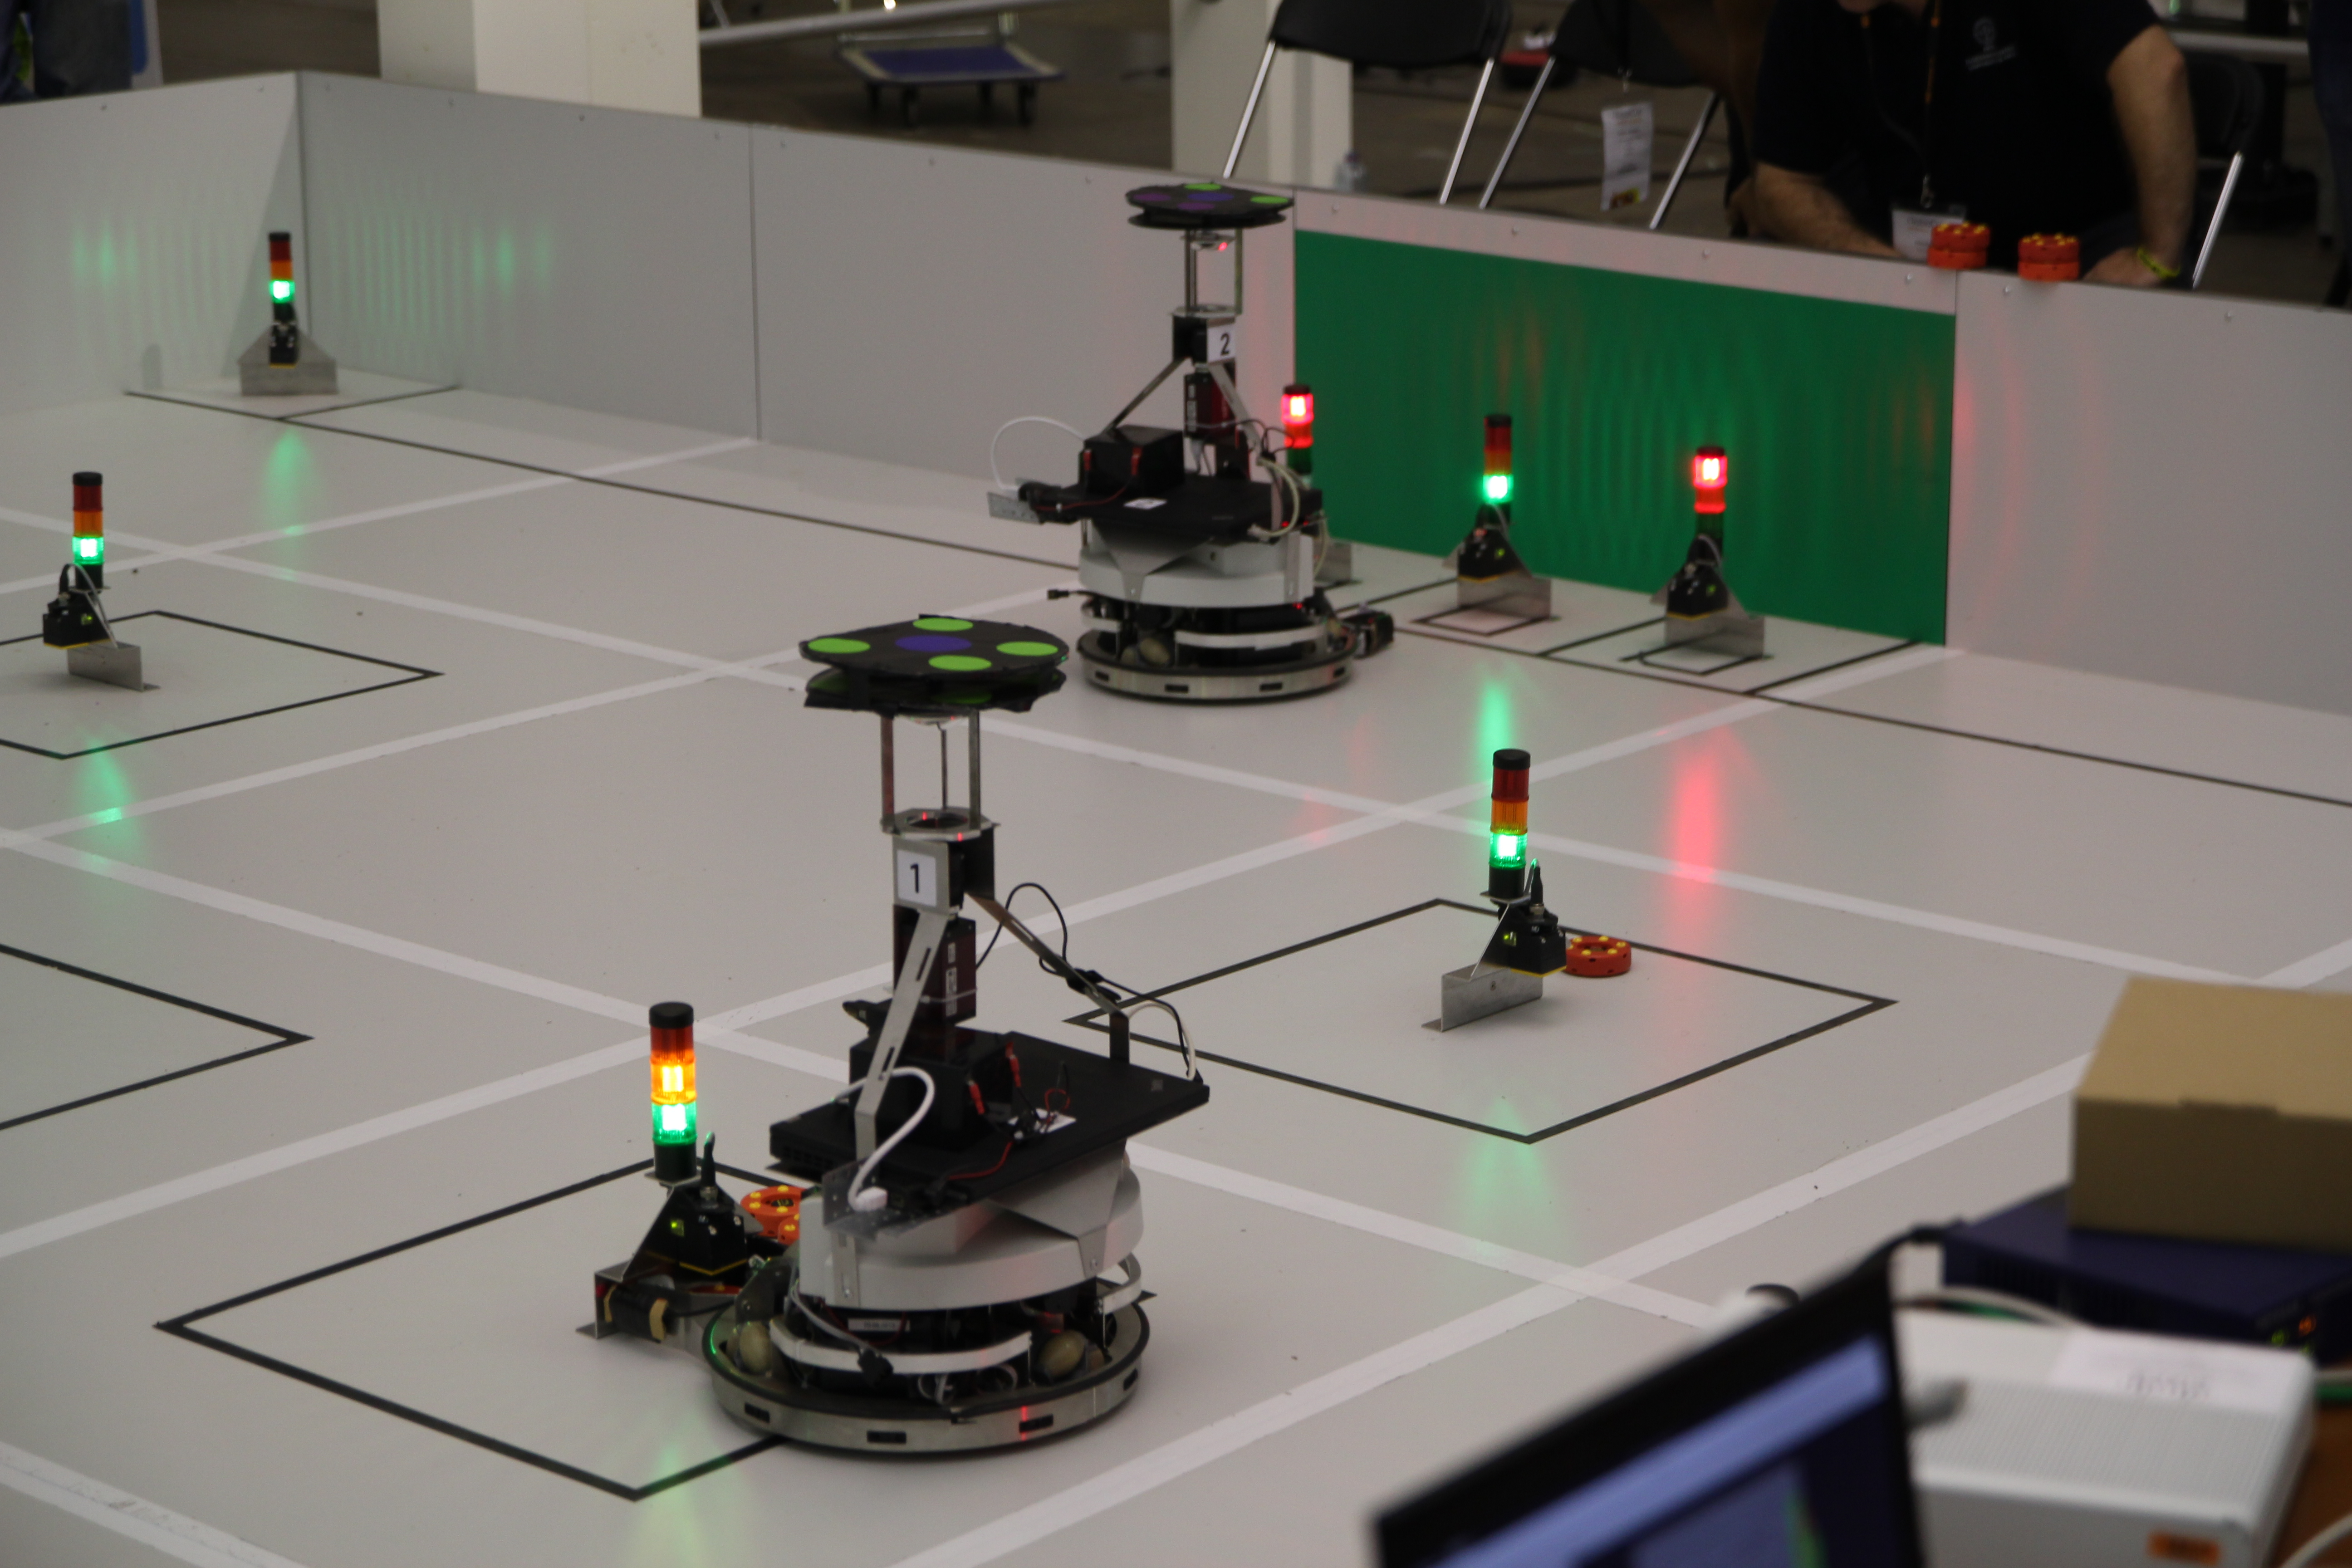
\includegraphics[scale=0.23]{pics/llsf}
\caption{Part of the LLSF field}
\label{fig:llsf_field}
\end{minipage}
\quad
\begin{minipage}[b]{0.5\linewidth}
\includegraphics[scale=0.45]{pics/production_chain}
\caption{LLSF Production Chain~\cite{LLSFRules}}
\label{fig:llsf_chain}
\end{minipage}
\end{figure}
Figure~\ref{fig:llsf_field} shows a part of the 5.6m x 5.6m hall with two Carologistics robots, three machines and some material-pucks. The main task of LLSF is to produce and deliver ordered products as efficiently as possible by feeding machines with resources and semi-finished products. The participants can use up to three Robotino robots by Festo~\cite{{Robotino}}. We present the Robotino in the next
section in detail. Orange pucks represent resources and products. They are equipped with an RFID-chip\footnote{Radio-frequency identification allows the wireless identification of objects with small chips.}
which is needed to store the different product states of the pucks. The machines are represented by the RFID-readers with signal-lights on top. The signal-lights indicate the current status of a machine, such as ``ready'', ``producing'' and ``out-of-order''. The machines need resources and semi-finished products as input and turn the last input puck into a further processed puck. All other input pucks are turned
into consumed pucks which can be recycled to produce new resource pucks. There are different types of machines. The type defines the needed input and the produced output of a machine. Figure~\ref{fig:llsf_chain} shows the production chain. There are the raw-material pucks $S_0$, intermediate product pucks $S_1$ and $S_2$ and product pucks $P_1$, $P_2$ and $P_3$. The machine types are labeled with
$T_1$ to $T_5$. Beside these regular machines, there are also recycling machines, which turn consumed pucks into raw-material pucks, and delivery machines which are used for delivering finished product pucks. Teams are awarded with points for delivering finished products, producing complex pucks and recycling. The game is divided into two phases. In the first phase, the \textit{exploration phase}, the robots have three minutes to explore the production area to identify which machine is of which type. Teams also receive points for each correctly reported machine-type. The second phase is the actual \textit{production phase} and lasts 15 minutes. The league also features an automated referee box (Refbox) which realizes the logic behind the LLSF environment. It controls machines and communicates with participating robots during the game. The Refbox gives orders which products are to be produced, informs the robots about the game state and rewards points for achieved goals.


\section{Robotino}
\label{sec:robotino}
\begin{figure}
\includegraphics[scale=0.11]{pics/carologistics_robotino}
\caption{A Robotino extended by Carologistics}
\label{fig:caro_robotino}
\end{figure}
The \textit{Robotino}~\cite{Robotino} is a mobile robot developed by Festo Didactic\footnote{\url{http://www.festo-didactic.com}}. It is used for research and education. The shape of the Robotino is a cylinder with 37cm diameter and 21cm height. It has omni-directional wheels to be able to drive in any direction and turn at the same time. It is equipped with nine infrared distance measuring sensors ordered around the robot, a bumper to detect collisions and a webcam. A micro-controller and an embedded PC with 500 MHz and 256 MB RAM are used to control the robot~\cite{Incremental}. The PC runs with a Linux Operating System. The Robotino is designed to be extendable to be used in different applications. Therefore additional sensors and actuators can be attached. At the front of the Robotino, there is a loading bay with some space for extensions. Figure~\ref{fig:caro_robotino} shows a Robotino extended by Carologistics. In addition to the default sensors shipped with the Robotino, we added a laser-rangefinder for localization and obstacle detection, a gyroscope and a framework which holds an omni-directional camera. The omni-directional camera consists of a camera facing upwards and a hyperbolic mirror above. The camera can see the whole area around the Robotino through the mirror. We adapted the omni-vision camera from former MSL-robots and now use it to detect LLSF pucks. The framework also holds a laptop connected to the Robotino, because we need more computational power than the Robotino provides for localization and path planning. We also attached a simple puck holder to the front. This puck holder is equipped with an infrared distance sensor to recognize if there is a puck in the holder and a digital optical sensor on each side of the puck holder. These are used to align the robot in front of LLSF machines. To observe the signal-lights on the machines, we use a webcam.\\


\section{Robot Software Frameworks}
\label{sec:robot_software_frameworks}
A robot software framework is a design and implementation which acts as a middleware and provides functionality and tools for the implementation of a robot control software~\cite{tnthesis}. In the following, we present Fawkes and ROS, which are the two robot software frameworks used in this thesis.

\subsection{Robot Operating System}
The \textit{Robot Operating System (ROS)}\footnote{\url{http://www.ros.org}} is an Open Source framework designed to operate on many robot platforms and to provide a standardized integration framework~\cite{Ros}. It provides a collection of useful Open Source libraries and tools for the development process of robot-software. Currently, it is widely used and has a large community. Each component integrated in ROS runs an own process and is called \textit{node}. ROS features peer-to-peer communication between nodes. Nodes can register a publisher or subscriber to a specified \textit{topic}. If a publisher of a topic sends a message, every subscriber of same topic receives the message. We will describe the message protocol Google Protobuf used by ROS later. The communication is managed by a process called \texttt{roscore}. \texttt{roscore} acts as a topic registry server. All nodes have to connect to the server in order to operate.\\
We use ROS in LLSF for two reasons. First, we use ROS for motion planning. The ROS package \texttt{move\_base} provides a global path planning and local motion planning with collision avoidance. We provide the position and orientation of the robot, laser data for obstacle detection and motion goals by publishing messages to specified topics. With this data, \texttt{move\_base} computes a motor command. We subscribe to the motor command topic and execute received commands. Second, we use the \texttt{rviz} package for visualization. For example, we visualize incoming laser data, the localization of the robot and motion plans. Moreover, we use \texttt{rviz} to send localization hints to the robot.

\subsection{Fawkes}
\textit{Fawkes}\footnote{\url{http://www.fawkesrobotics.org}} is an Open Source robot software framework developed primarily at the Knowledge-based Systems Group\footnote{\url{http://www.kbsg.rwth-aachen.de}} (KBSG) at RWTH Aachen University~\cite{FawkesDesign}. It is designed to run on multiple platforms and domains. It is written for Unix systems and follows a component-based software design~\cite{component}. It provides an infrastructure to load and unload binary components (implemented as \textit{plugins}) at run-time. Fawkes features a \textit{blackboard} as communication structure between plugins. The blackboard lists structured entries called \textit{interfaces}. Plugins are composed of thread, which can read and write interfaces with a specified id. There can be many readers but only one writer for an interface. Furthermore, Fawkes organizes plugin activity in threads to make use of multi-core architectures. Because of this design, Fawkes is flexible and dynamic. The interchangeability of the plugins, which is caused by well defined interfaces, makes hardware abstraction and reuse easy. This is also an important advantage for the development of the simulation because the simulation can easily exchange lower-level robot control and sense plugins. Then, robot control plugins on higher levels can operate as on the real robot because the interface is the same. The features of Fawkes are provided as \textit{aspects}. These aspects are based on aspect-oriented programming~\cite{aspect_oriented} and give access to a particular feature. Threads that want to use a feature can inherit from the corresponding aspect. For example there are aspects for accessing the blackboard, logging and timing~\cite{tnthesis}. In this thesis, we give access to communication with the simulation by providing such an aspect. Two other important features for this thesis are the centralized clock and the configuration. The centralized clock provides the time for all plugins. Especially important for this thesis is the possibility to give Fawkes an alternative time-source. So, it is easy to exchange the system time with the simulation time for all plugins without having to modify them. Also important for this thesis is the way Fawkes provides configurations. The configuration-files for all plugins are described in the same format. A super-ordinate configuration file chooses which configuration files have to be loaded. There is the possibility to start Fawkes with a specified configuration by setting a super-ordinate configuration file. Furthermore, Fawkes features a behavior engine. A behavior called \textit{skill} is formalized by a hybrid state machine and implemented in the scripting language Lua~\cite{behavior_engine}.\\
In comparison to ROS, the advantage of Fawkes is the tighter integration of the used components. The main loop of Fawkes controls the execution order of all component threads. This enables matching certain time criteria for the components and to provide a \textit{sense-think-act} cycle. We use Fawkes as our main robot software framework. Nearly all software components for our robot are integrated as plugins into Fawkes. Therefore, we have to provide sensor data from the simulation and get actuator-commands in Fawkes.

\section{Gazebo}
\label{sec:gazebo}
Gazebo\footnote{\url{http://gazebosim.org}} is an Open Source robot simulator~\cite{GazeboDesign}. It provides a platform to simulate all kinds of robots with sensors and actuators and their environment in a three dimensional world. It runs on UNIX and is written in C++. Originally, Gazebo was designed for large outdoor environments, but it is well suited for indoor environments, too. The development was started as part of the Player/Stage project~\cite{PlayerStage} and was an alternative to the two dimensional simulator stage. Gazebo became independent later. Now, it has a strong relation to ROS and is even available as a package in ROS. Gazebo is an frequently used simulator. It is, for example, the simulator chosen for the recently held Virtual Robotics Challenge founded by DARPA. We present the use of Gazebo in this challenge in the related work.\\
Gazebo uses proven Open Source engines for graphical presentation and physics. \textit{Ogre}\footnote{\url{http://www.ogre3d.org}} is the graphic engine used in Gazebo. It allows rendering graphically realistic environments with reflections, shadows and detailed textures. This is important for the simulation of camera sensors because often reflections of light sources and inconstant lighting can cause problems. Gazebo uses the \textit{Open Dynamics Engine (ODE)}~\footnote{\url{http://www.ode.org}} and \textit{Bullet}~\footnote{\url{http://bulletphysics.org}} to simulate physical interactions between objects. It features an abstraction layer for physics and can therefore use both physic engines interchangeably. Bullet features lower computation cost and more complex shapes than ODE, whereas ODE has a larger documentation and background in robot simulators. Furthermore, the abstraction layer for the physics engine allows the access to detailed parameters of the engines.\\
A simulation in Gazebo consists of different elements: \textit{Models} describe physical objects in the simulation, such as a table or a robot. The model is built out of \textit{joints} and \textit{links} which consist of a number of geometries. These geometries can either be visible objects or collision objects used for physics. Joints connect two links and define the possible motion of the links in relation to each other. For example, joints are used to define axes of wheels. Furthermore, a model can contain sensors which are represented by a set of properties to define the sensor. A \textit{world} describes the whole simulation environment in Gazebo. It consists of models and light sources. It also has a range of properties for the physics simulation, rendering and the general simulation. Models and Worlds can be defined in an XML-like format called \textit{Simulation Description Format (SDF)} which is based on the \textit{Unified Robot Description Format (URDF)} of ROS but is optimized for the use in a simulation. Beside the physical description of objects in the simulation there are also \textit{plugins} in Gazebo to modify the simulation at run-time. These plugins belong to a model, a sensor or a world. They use the Gazebo application programming interface (API) to model the behavior of different objects. For example, there are plugins for robot models, which apply motion to the corresponding model if the robot receives a movement order, and plugins for the world, which can spawn new models.\\
Out of the box, Gazebo includes a variety of generalized sensors and models of common robots and other objects such as tables, cups and even buildings. For example, there are robot-models for the PR2 by Willow Garage, Atlas by Boston Dynamics and the Kuka YouBot. In the Gazebo framework, there is basic support for a set of general sensors. This includes cameras, contact-sensors, GPS, inertia measurement units, laser sensors and sonar sensors. The support of all these common sensors and models allows easy development of a specific simulation environment. Not included models, sensors and plugins can be added and fit well in the existing context.\\


\section{Additional Tools}
\label{sec:additional_software}
In this section, we present Protocol Buffers and CLIPS, which are two additional tools that are important for the thesis.

\subsection{Protocol Buffers}
For communication between Fawkes and Gazebo, we use \textit{Protocol Buffers (Protobuf)}\footnote{\url{https://developers.google.com/protocol-buffers}}, a data interchange format developed by Google. Protobuf serializes data in a pre-defined structure for efficient data transportation and storage. It is flexible and language-independent. The data structure is hierarchical and dynamic and can be implemented in a simple specification language. Protobuf then uses this data structure to generate code in a specified programming language. The code is able to efficiently serialize and deserialize data. The generation of code in the different languages makes it easy to include Protobuf in an implementation. The data structures are kept simple and can be built hierarchically. In the following, we use the term type to refer to the data structure behind a Protobuf message. Because of its efficiency and simplicity, Protobuf is widely used. Especially ROS, Gazebo, the LLSF Refbox and our agent use Protobuf to transport messages.

\subsection{CLIPS Rules Engine}
We implemented our high level control agent with the \textit{CLIPS} rules engine\footnote{\url{http://clipsrules.sourceforge.net}}. It is an expert system developed by NASA\footnote{National Aeronautics and Space Administration (NASA) of the USA} with rule-based, object-oriented and procedural programming paradigms~\cite{Clips,clips_manual}. It basically consists of a ~\textit{fact base}, a \textit{knowledge base} and an \textit{inference engine}. The fact base acts as working memory~\cite{Incremental}. \textit{Facts} in the fact base represent pieces of information and can be unstructured or structured by a template. The knowledge base consists of \textit{rules} and \textit{functions}. Rules represent heuristic knowledge and are the basic part of the expert system. They are composed of an \textit{antecedent} and a \textit{consequent}. The antecedent contains a set of conditions. If all conditions of the antecedent can be matched by the fact base, the rule is applicable. The consequent contains a set of actions which are executed if a rule is applied. For example, these actions can assert new facts to the fact base or delete existing ones. Functions represent procedural knowledge. The inference engine realizes a forward-chaining mechanism based on the Rete algorithm~\cite{rete}. It matches the fact base to the antecedent of the rules to determine which rules are applicable. Then, it decides which applicable rule to execute by a priority defined in the rules. After executing the rule and probable changes to the fact base, the whole method is repeated until no more rules are applicable. A special feature of CLIPS is the integration into other programming languages. Other languages can dynamically assert facts in CLIPS and CLIPS can call functions from this language. This integration makes CLIPS a good choice for the control of an embedded system.

%% \subsection{MongoDB}
%% \textit{MongoDB}\footnote{\url{http://www.mongodb.org}} is an Open Source, document-oriented database~\cite{mongodb,KlingenDA}. The basic elements in MongoDB are documents. Documents are grouped in so called collections which are contained in a database. Documents contain a set of key-value pairs, can be nested and are schema-free. This means that there are no constraints to the keys in a document. This provides a flexible and simple use. MongoDB uses indexing to increase querying speed. \textcolor{red}{cut off MongoDB section or better description?}\\
%% In this thesis, we use MongoDB to store statistics about simulated LLSF games. MongoDB also gives us the possibility to log sensor data and the belief and decisions of the agents~\cite{KlingenDA}.

\chapter{Related Work}
In this chapter we present work related to this thesis. In section 3.1, we descibe alternatives to Gazebo and why we choose Gazebo. In section 3.2, we give an overview of other popular simulations, especially a simulation that also uses Gazebo and other multi-robot simulations, and in section 3.3, we describe our current multi-robot strategy as well as other attractive strategies our simulation should be able to evaluate. In the following, we will use the terms \textit{multi-robot} and \textit{multi-agent} interchangeably because the common term in litrature is multi-agent and we want to use multi-robot. A multi-agent system can consist of fully abstract agents, such as \textcolor{red}{...}, whereas we are dealing with multi-robot system and therefore robots that interact physically with their environment.


\section{Other Simulators}
\subsection{Stage}
\subsection{Webots}
\subsection{USARSim}
\subsection{Simspark}
\subsection{Robotino Sim Professional}
\subsection{Choice for Gazebo}

\section{Simulations}
\subsection{Virtual Robotics Challenge}
\subsection{RoboCup Simulation Leagues}
\subsection{Simulation Environment for the Middle Size League}

\section{Multi-Agent Strategies}
\subsection{Incremental Task-level Reasoning}
\subsection{Marked Based Strategies}

\chapter{Approach}
In this chapter, we describe the approach of this thesis by presenting the main ideas to reach our goals for the simulation in section 4.1. In section 4.2, we present the architectural approach.

\section{Goals and Approaches}
\textbf{Realistic simulation:} The realism of the simulation is an important goal of the thesis. A more realistic simulation allows better testing because the simulation is more similar to the reality. Therefore more problems of reality can be simulated. The reality of the simulation has many different aspects. The first group of aspects belong to the realism of the sensor data. There are some sensors that are easy to simulate, such as distance sensors, bumpers and gyroscopes. Others, especially cameras, are more difficult to simulate realistically. The choice of Gazebo with ODE and Ogre for the visual appearance already allows us to simulate a wide range of sensors realistically. An other aspect for the realism is noise in the sensor data. For all metric sensors, we simulate this as Gaussian noise with the calculated value as mean and a configurable variance. The second group of aspects belong to the realism of the physical environment. Objects have to behave in the simulation and the reality in a similar way. This is especially important for robot movement and manipulation tasks. Here Gazebo with ODE also provides high realism out of the box. Nevertheless, it is important to find good physical parameters for the simulated objects. Examples of those parameters are the mass and coefficients of friction. An other important aspect of realism is that the simulation should not introduce new problems which do not occur in reality. Such a problem, which occurred in the development of the thesis, is that the simulation ran slower than the system time.\\
\textbf{Different levels of simulation:} Besides a simulation, which is so realistic as possible, it is also useful to test with a more abstract simulation. This allows testing the optimal case without sensor noise or without using low level components, such as localization, if those produce new errors or are not finished jet. To be able to simulate on different levels we use the multi-level abstraction approach presented in the chapter about related work. Where we use multiple abstraction levels is shown in the next section about the architecture.\\
\textbf{Compatibility with original robot software:} We want to achieve the goal that the robot software runs in the simulation in the same way as in reality. This is important because otherwise it would result in additional effort to keep the robot software in the simulation and in the reality running and this effort can cause more difference between simulation and reality. In the thesis, the simulation should use the same interfaces as the real components that are simulated. In Fawkes this is easy to achieve because the interfaces between components are well defined and components using an interface do not recognize whether the interface is provided by the simulation or a real component. \textcolor{red}{woerter zu oft wiederholt?}\\
\textbf{Efficient testing:} We want to make the use of the simulation as efficient as possible. To achieve this, we provide the following features. We provide scripts which automatically start the full simulation with all needed programs. Without this scripts, it would take much time. For a full simulation of an LLSF game, it is necessary to start Gazebo, the Refbox, a controlling Fawkes instance and, for the Robotinos, three times Fawkes, Roscore and Movebase\footnote{Movebase is the ROS program we currently use for navigation with collision avoidance.}. Each program-instance has to be started with correct parameters.  An other approach we use to increase the efficiency is the feature to load different configurations and setups. For example, the scripts provide the possibility to load the simulation with different numbers of Robotinos, abstraction levels and simulation environments. Loading different configurations for the robot software is a feature of Fawkes and useful for us. We also integrated this in the scripts. We also provide the possibility to draw objects into the simulation. This makes it easy to visualize the belief and intentions of a robot to identify mistakes or ways to improve the system~\cite{Visualization}.\\
\textbf{Multi-robot system evaluation:} An important part of this thesis is the evaluation of multi-robot systems. The features we already mentioned in the previous paragraph are here especially useful because the testing effort (e.g. to setup the simulation or analyzing the cooperation between robots) often scales with the number of robots. To evaluate the performance of the multi-robot system faster without having to observe the simulation all the time, we provide the possibility to run multiple simulation runs, in our case runs of LLSF games, automatically. With this feature, the simulation can run for example 20 times over night. To analyze the executed simulation runs, we keeps statistics of each run. For our LLSF domain, we keep the amount of achieved points with a detailed list of all actions which gave points at which time. These statistics can easily be extended by the amount of collisions between robots, waiting time for resource locks or other useful measurements. Sometimes it can happen that single simulation runs have a very different result. To find the reason for this result, we keep the log files of the run and also record the simulation itself. With this record, the simulation run can be reconstructed. The record contains the position and movements of all objects in the simulation. Here it is also useful to draw additional information, such as the localization of the robots, in the simulation to be able to analyze faults without having to look in the log files. The automated simulation runs also allow the comparison of different configurations of the multi-robot system. The automation script can be started with a number of configurations that are all tested. This can be useful for finding the best performing role combination or parameters such as thresholds.\\
\textbf{Expendability and flexibility:} An essential criterion of a good simulation is the expendability to adapt to future changes. On the one hand, there will be changes to the Carologistics Robotino and to LLSF. These changes have to be easy to implement in the simulation, otherwise the simulation would not remain useful. On the other hand, it is attractive to use the simulation also in other domains, such as RoboCup @Home. To achieve the expendability of the simulation, we provide a framework for simulated devices in Gazebo and Fawkes. Furthermore we concentrate on developing small modules that are exchangeable and reusable. In Gazebo, new modules can easily be added to the robot and world plugins. In Fawkes it is easy to implement a new plugin which provides the wanted features because the plugin can use the provided Gazebo aspect. In addition, a detailed documentation and example plugins allows other developers to easily extend the simulation. \textcolor{red}{TODO: wiki plugin dev!}. The simulation should also be flexible to adapt to small changes. Therefore we provide several configuration files for the simulation environment, the simulated objects and robots and the plugins for Gazebo and Fawkes. \textcolor{red}{Gazebo config}



\section{Architecture}

\chapter{Implementation}
\label{cha:implementation}
In this chapter, we describe how we implemented the simulation. First, section~\ref{sec:modules} presents the various modules we developed by describing what their task is, what we noticed during the implementation and why we implemented it this way. \textcolor{red}{module dependencies extra or in modules?} In section~\ref{sec:module_dependencies}, we describe the dependencies and interaction between the modules we developed. Section~\ref{sec:imp_communication} covers the implementation of the communication between Fawkes and Gazebo and between multiple robots we want to simulate. In section~\ref{sec:agent_improvements}, we present the improvements for the multi-agent system we implemented during the thesis.

\section{Modules}
\label{sec:modules}

\section{Module Dependencies}
\label{sec:module_dependencies}

\section{Communication}
\label{sec:imp_communication}

\section{Agent Improvements}
\label{sec:agent_improvements}
dynamic role switch: no more products ordered, \cite{dynamic_role_assignment}

\chapter{Evaluation}
\label{cha:evaluation}

This is the evaluation.


Expendability: hackathon, Ceasar?

realism: time error?

bad network influence eval

\chapter{Summary and Future Work}
\label{cha:summery_and_future_work}
In this chapter, we conclude the thesis in section~\ref{sec:summery} and give an outlook to possible future work on the simulation and our multi-robot system for LLSF in section~\ref{sec:future_work}.

\section{Summary}
\label{sec:summery}
In this thesis, we have developed a multi-robot simulation for the LLSF. The simulation was designed to allow for efficient testing of multi-robot coordination and and other important parts of multi-robot systems. We achieved this by implementing a realistic LLSF simulation in Gazebo and connecting this simulation to Fawkes. In Fawkes, simulation plugins replace real sensor and actuator plugins and provide the same blackboard-interfaces so that the components we want to test can operate in the same way as on a real robot. To increase efficiency during testing and evaluation, we implemented start-up scripts and automated test runs with statistics and reconstructions of simulated runs. The simulation also was designed and implemented in a way to simplify the implementation of future changes of the LLSF and the Carologistics Robotino. This also allows using the simulation in other domains and with other robots because the small plugins and modules we implemented can be reused. For better testing possibilities, we included multi-level abstraction which allows us to test high level components with either simulated sensor data or ground truth information. \\
To improve our multi-agent system and test the evaluation capabilities of the simulation, we implemented a dynamic role change to adapt the task allocation to the situation and recycling to score more points more continuously during the production of complex products. Furthermore, we extended our previous role-based approach to work with three instead of two robots in the exploration and production phases.\\
We evaluated how realistic our simulation is. Limitations of the simulation realism are mainly caused by missing visual phenomenons, such as realistic reflections, and finding realistic physical properties, such as friction parameters. Despite these limitations, we can realistically simulate the LLSF environment as well as sensors and actuators of the Robotino, what is more than sufficient for the purpose of evaluating our multi-robot systems.\\
In the evaluation, we analyzed the performance of several configurations with different role assignments and agent improvements. We found that two $P_3$ agents perform significantly better than other configurations because producing $P_3$ pucks continuously provides many points has the least likelihood to fail. Recycling improved the performance of the system because it provides points early in the production process of a complex product. However, it also added more steps to the production process what increased the likelihood to fail at some point during the production. The dynamic role change provided a smaller advantage than we expected because the role change happens only late and rarely. The performance of all configurations was limited by the several problems we identified in the evaluation. These problems mainly include navigation coordination, reliability of low level movement and failure handling. We noticed that these problems have to be solved before improvements on the high level agent can use their full potential. These problems especially limit the performance of configurations with three robots as we showed in the evaluation.\\
During the Bonding Hackathon, about 40 people successful developed skills, that work in reality, by mainly using our simulation as test platform. This showed that our simulation is very useful in the development process of robot software, even for users unexperienced in developing on robot systems. It also showed that our simulation is extendable for use in other domains with other sensors. The simulation has also been successfully used in the development of the vision detection for the Hackathon and the testing of an alternative navigation and collision avoidance plugin on the Robotino.

\section{Future Work}
\label{sec:future_work}
In the near future, the simulation and our multi-robot system solution for LLSF need to be changed because LLSF is going to be changed~\cite{llsf_changes}. At the RoboCup 2014, it is likely that two teams play at the same time on the same field with double size. The machines with RFID-readers might get replaced by small assembly machines. This also demands hardware changes on the Robotino, such as adding a new gripper. We probably also add different sensors in the near future, such as a stereoscopic camera to the Robotino to get a more reliable puck and light-signal detection. The simulation and the agent have to be adapted to these changes.\\
The simulation can also be extended to work in other domains with other robots, such as domestic service robots. The motor and basic sensors we implemented can be reused for this. To improve the expandability of the simulation even further, it is also useful to refactor the Gazebo plugins. Existing modules for sensors and actuators can be separated into different plugins. This would allow reconfiguration and building new simulated robots without recompiling. Two other small improvements we want to implement in the future are the simulation of the omnivision-camera and providing the simulation-time in ROS for more realistic \texttt{move\_base} results.\\
The simulation developed in this thesis can be the foundation of a variety of future projects. For example, the visualization possibilities could be used to visualize agent belief and intention. This would simplify the development of more advanced agent strategies. Another interesting extension of the simulation would be using the automatic simulation runs to implement some kind of machine learning or parameter finding. The simulation is an important tool for future development for the LLSF. In the near future, we have to solve the problems we discovered in section~\ref{sec:multi_robot_strategies}. This includes navigation-coordination with multiple robots to avoid that two robots block each others path, improving the locking approach to be more robust against failure, increasing reliability of low level skills and recovery from situations shown in Figure~\ref{fig:fails}. To improve the performance of our multi-robot system, we also have to develop large agent improvements. Such an improvement could be a more flexible task allocation strategy, such as Murdoch. It would allow us to optimize the task allocation and produce complex products faster because we could divide tasks in smaller pieces.


%reenable empty pages before chapter
\let\cleardoublepage\cleardoublepage

\newpage

\bibliographystyle{plain}
\bibliography{references}

\end{document}
